\documentclass[a4paper,12pt]{article}
\usepackage[framed,numbered,autolinebreaks,useliterate]{mcode}
\usepackage{CJKutf8}
\setlength{\headheight}{15pt} 
\usepackage{textcomp}
\usepackage{amsmath}
\usepackage{amssymb}
\usepackage{listings}
\usepackage{float}
\usepackage{xcolor}
\usepackage{color}
\usepackage{fancyhdr}
\usepackage{lastpage}
\usepackage{times}
\usepackage{mathptmx}
\usepackage{geometry}
\usepackage{booktabs}
\usepackage{graphicx}
\geometry{left=3.17cm,right=3.17cm,top=2.54cm,bottom=2.54cm}
\usepackage{indentfirst}
\setlength{\parindent}{2em}
\rhead{Page \thepage{} of \pageref{LastPage}}



\begin{document}
\begin{CJK*}{UTF8}{gbsn}



\section{实验课题}
下面利用蒙特卡罗方法计算一个冰淇淋的体积和质量.\par
假设冰淇淋的下部为一锥体而上部为一个半球, 锥面方程为$z^2=x^2+y^2$, 球面方程为$x^2+y^2+(z-1)^2=1$. 完成以下实验:\par 
\begin{enumerate}
\item 画出冰淇淋的图形.
\item 分别用确定性方法和蒙特卡罗方法计算冰淇淋的体积, 比较计算结果.
\item 假设冰淇淋的密度函数为为$f(x,y,z)=z\exp{[-(x^2+y^2+z^2)]}$, 分别用确定性方法和蒙特卡罗方法计算冰淇淋的质量, 比较计算结果.
\end{enumerate}



\section{图形绘制}
联列两曲线方程我们可以得到冰淇淋图形以平面$z=1$为分界面, 上部分为半球, 下部分为圆锥.\par\vspace{10pt}
\noindent 对于圆锥, 因为$z\geqslant0$, 所以我们有$z=\sqrt{x^2+y^2}$. 绘制圆锥的程序如下:\par\vspace{-15pt}
\begin{lstlisting}
z1 = @(x,y) sqrt(x.^2+y.^2);
g1 = ezmesh(z1,[-1/sqrt(2),1/sqrt(2),-1/sqrt(2),1/sqrt(2)],'circ');
\end{lstlisting}\vspace{10pt}
\noindent 对于半球, 因为$z\geqslant1$, 所以我们有$z=\sqrt{1-x^2-y^2}+1$. 绘制半球的程序如下:\par\vspace{-15pt}
\begin{lstlisting}
z2 = @(x,y) sqrt(1-x.^2-y.^2)+1;
g2 = ezmesh(z2,[-1/sqrt(2),1/sqrt(2),-1/sqrt(2),1/sqrt(2)],'circ');
\end{lstlisting}\vspace{10pt}
冰淇淋图形的绘制结果如\textbf{图1}.\par
\begin{center}
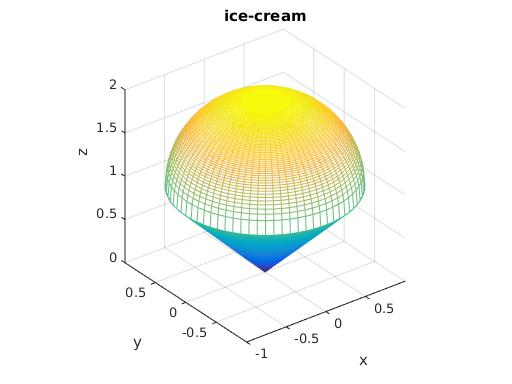
\includegraphics[width = 11cm]{ice_cream.jpg}\\
\textbf{图1} 冰淇淋示意图\\
\end{center}



\section{体积计算}

\subsection{精确解}
我们引入球坐标, 则$x=r\sin{\theta}\cos{\phi}$, $y=r\sin{\theta}\sin{\phi}$, $z=r\cos{\theta}$. 其中$\theta$为球面上的点与$z$轴正向的夹角, $\phi$为平面$xOy$上的点与$x$轴正向的夹角. 利用球面三重积分我们可以得到冰淇淋的体积
\begin{equation*}
V=\int^{}_{\omega}{\rm d}x{\rm d}y{\rm d}z=\int^{2\pi}_{0}\int^{\pi/4}_{0}\int^{2cos{\theta}}_{0}r^2\sin{\theta}{\rm d}r{\rm d}\theta{\rm d}\phi.
\end{equation*}
下面是求冰淇淋体积的\textsc{Matlab}程序.\par\vspace{-15pt}
\begin{lstlisting}
V1 = eval(int(int(int(r*r*sin(theta),r,0,2*cos(theta)),...
    theta,0,pi/4),phi,0,2*pi));
\end{lstlisting}\par
上面程序的计算得到的体积为3.141593. 事实上, 如果我们去掉上面代码中的eval函数, 在\textsc{Matlab}软件的控制台中显示的计算结果就是pi.
\subsection{近似解}
首先, 冰淇淋可以被装在如下的立方体区域内:
\begin{equation*}
-1 \leqslant x \leqslant 1, -1 \leqslant y \leqslant 1, 0 \leqslant z \leqslant 2.
\end{equation*}\par
接下来我们在这个体积为8的立方体区域中生成随机点. 若我们共生成了$N$个随机点, 其中有$m$个落在了冰淇淋区域内, 那么冰淇淋的体积$V$可以被表示为
\begin{equation*}
V=\frac{8m}{N}.
\end{equation*}
下面是上述方法的\textsc{Matlab}实现.\par\vspace{-15pt}
\begin{lstlisting}
countAll = 1000000;
countInIceCream = 0;
for i = 1:countAll
   w = [2*rand(1)-1,2*rand(1)-1,2*rand(1)];
   if (w(3)^2>w(1)^2+w(2)^2 && w(1)^2+w(2)^2+(w(3)-1)^2<1)
       countInIceCream = countInIceCream + 1;
       %S = S + f(w(1),w(2),w(3));
   end
end
V2 = 8 * countInIceCream / countAll;
\end{lstlisting}\par
由于我们使用了随机数, 上面的程序的计算结果具有不确定性, 但根据概率统计原理我们知道, countAll越大, 我们的计算结果越倾向于靠近$\pi$.本次实验中我们取countAll的值为1000000,得到冰淇淋的近似体积3.141360.
\section{质量计算}
\subsection{精确解}
我们再次使用球坐标变换,并把冰淇淋的密度函数$f(x,y,z)=z{\rm e}^{-(x^2+y^2+z^2)}$转换为$g(r,\theta,\phi)=r\cos{\theta}{\rm e}^{-r^2}$. 对冰淇淋区域内的密度函数积分, 我们可以得到冰淇淋的质量
\begin{equation*}
M=\int^{}_{\omega}f(x,y,z){\rm d}x{\rm d}y{\rm d}z=\int^{2\pi}_{0}\int^{\pi/4}_{0}\int^{2cos{\theta}}_{0}r^2\sin{\theta}g(r,\theta,\phi){\rm d}r{\rm d}\theta{\rm d}\phi.
\end{equation*}\par
下面是求冰淇淋质量的\textsc{Matlab}程序. 从而我们得到冰淇淋质量的精确解为0.615969.\par\vspace{-15pt}
\begin{lstlisting}
M1 = eval(int(int(int(r^3*sin(theta)*cos(theta)*exp(-r^2),...
    r,0,2*cos(theta)),theta,0,pi/4),phi,0,2*pi));
\end{lstlisting}\par

\subsection{近似解}
与估算体积时的方法类似,我们在立方体区域中随机生成$N$个点. 首先我们用落在冰淇淋区域中的点来估计冰淇淋的平均密度, 接着我们估计的密度和之前估算的体积求得冰淇淋的质量.\par
如果有$m$个点落在冰淇淋区域内, 记第$i$个这样的点为$P_i$, 则$P_i(x_i,y_i,z_i)$处的密度为$f(x_i,y_i,z_i)$. 所以我们可以得到这$m$个点的平均密度
\begin{equation*}
\rho=\frac{\sum_{i=1}^{m}f(x_i,y_i,z_i)}{m}.
\end{equation*}\par
用$\rho$代替冰淇淋的实际密度, 再带入估计得到的冰淇淋体积$V$, 我们可以得到冰淇淋质量的表达式\par
\begin{equation*}
M=\rho V=\frac{\sum_{i=1}^{m}f(x_i,y_i,z_i)V}{m}.
\end{equation*}\par\vspace{5pt}
\noindent 下面的\textsc{Matlab}程序实现了上述算法, 并得到0.615819的质量估算结果.\par\vspace{-15pt}
\begin{lstlisting}
S = 0;
f = @(x,y,z) z*exp(-(x^2+y^2+z^2));
for i = 1:countAll
   w = [2*rand(1)-1,2*rand(1)-1,2*rand(1)];
   if (w(3)^2>w(1)^2+w(2)^2 && w(1)^2+w(2)^2+(w(3)-1)^2<1)
       %countInIceCream = countInIceCream + 1;
       S = S + f(w(1),w(2),w(3));
   end
end
M2 = S / countInIceCream * V2;
\end{lstlisting}\par
\section{实验结论}
本实验以一个简单的冰淇淋图形为研究对象, 考察了用蒙特卡罗方法求积分的近似值.\par
在本次实验中, 使用蒙特卡罗方法得到的计算结果相对误差较小: 当随机点个数达到百万级别时, 相对误差基本控制在0.05\%以下.

\section{附录}
\noindent\textbf{Lab03.m} 源代码
\vspace{-10pt}
\lstset{basicstyle=\ttfamily\footnotesize,escapechar=`}
\begin{lstlisting}
%Lab03.m
clear;clc;format long;
syms theta r phi;
countAll = 1000000;
countInIceCream = 0;
S = 0;
f = @(x,y,z) z*exp(-(x^2+y^2+z^2));

%draw the figure
z1 = @(x,y) sqrt(x.^2+y.^2);
figure('name','ice-cream figure');
g1 = ezmesh(z1,[-1/sqrt(2),1/sqrt(2),-1/sqrt(2),1/sqrt(2)],'circ');
hold on;
z2 = @(x,y) sqrt(1-x.^2-y.^2)+1;
g2 = ezmesh(z2,[-1/sqrt(2),1/sqrt(2),-1/sqrt(2),1/sqrt(2)],'circ');
title('ice-cream');
axis equal;

%generate random points
for i = 1:countAll
   w = [2*rand(1)-1,2*rand(1)-1,2*rand(1)];
   if (w(3)^2>w(1)^2+w(2)^2 && w(1)^2+w(2)^2+(w(3)-1)^2<1)
       countInIceCream = countInIceCream + 1;
       S = S + f(w(1),w(2),w(3));
   end
end

%calculate volume
V1 = eval(int(int(int(r*r*sin(theta),r,0,2*cos(theta)),...
    theta,0,pi/4),phi,0,2*pi));
V2 = 8 * countInIceCream / countAll;
fprintf('The actual volume of the ice-cream is %.6f.\n\n',V1);
fprintf('The estimated volume of the ice-cream is %.6f.\n\n',V2);


%calculate mass
M1 = eval(int(int(int(r^3*sin(theta)*cos(theta)*exp(-r^2),...
    r,0,2*cos(theta)),theta,0,pi/4),phi,0,2*pi));
M2 = S / countInIceCream * V2;
fprintf('The actual mass of the ice-cream is %.6f.\n\n',M1);
fprintf('The estimated mass of the ice-cream is %.6f.\n\n',M2);
\end{lstlisting}




\end{CJK*}
\end{document}
